\begin{figure*}[t!]
  \centering
  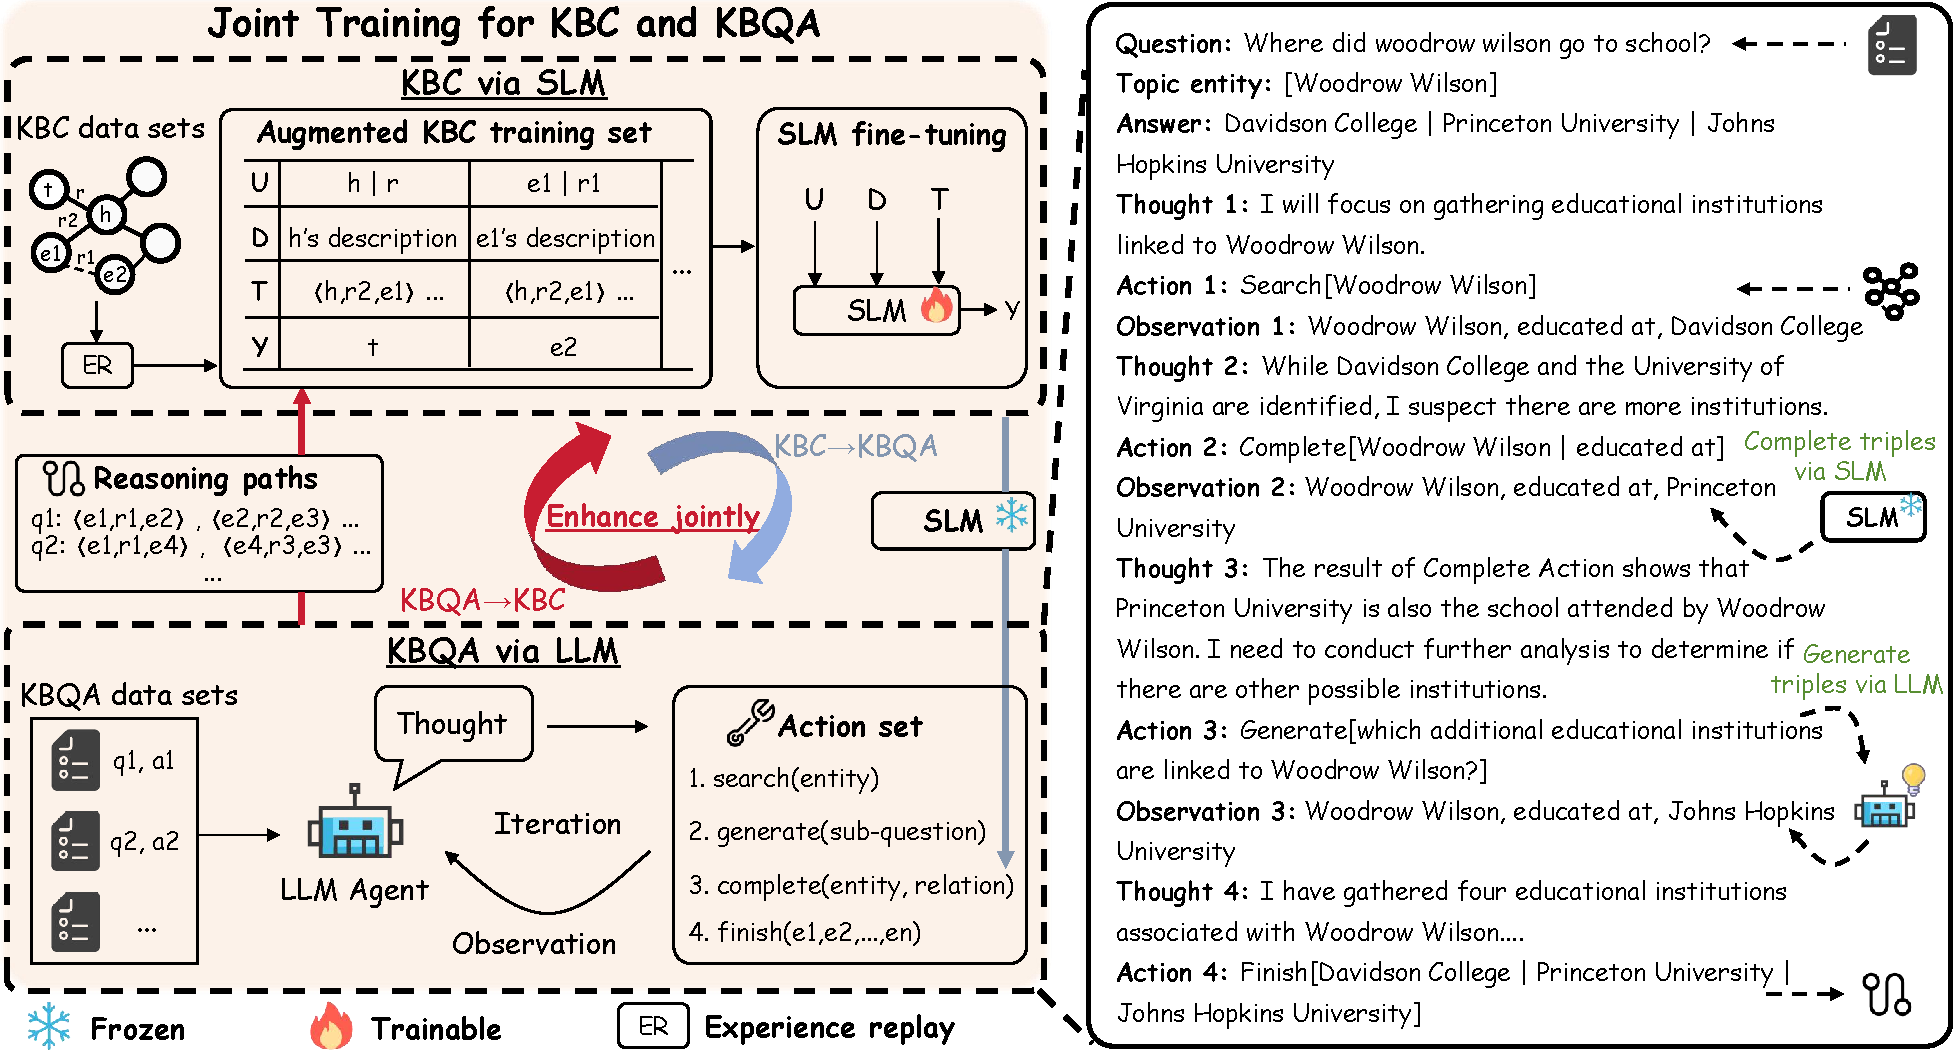
\includegraphics[width=0.96\linewidth]{image/img/Model_overview.pdf}
    % \setlength{\abovecaptionskip}{-0.5mm}
    % \setlength{\belowcaptionskip}{-2mm}
  % \vspace{-4pt}
  \caption{Overview of our framework JCQL.}
  % \vspace{-4pt}
  \label{Framework overview}
\end{figure*}


% subgraph
% \begin{figure*}[htb!]
%     \centering
%     \subfigure[Fine-tune]{
%         \label{model overview:subfig:onefunction}
%         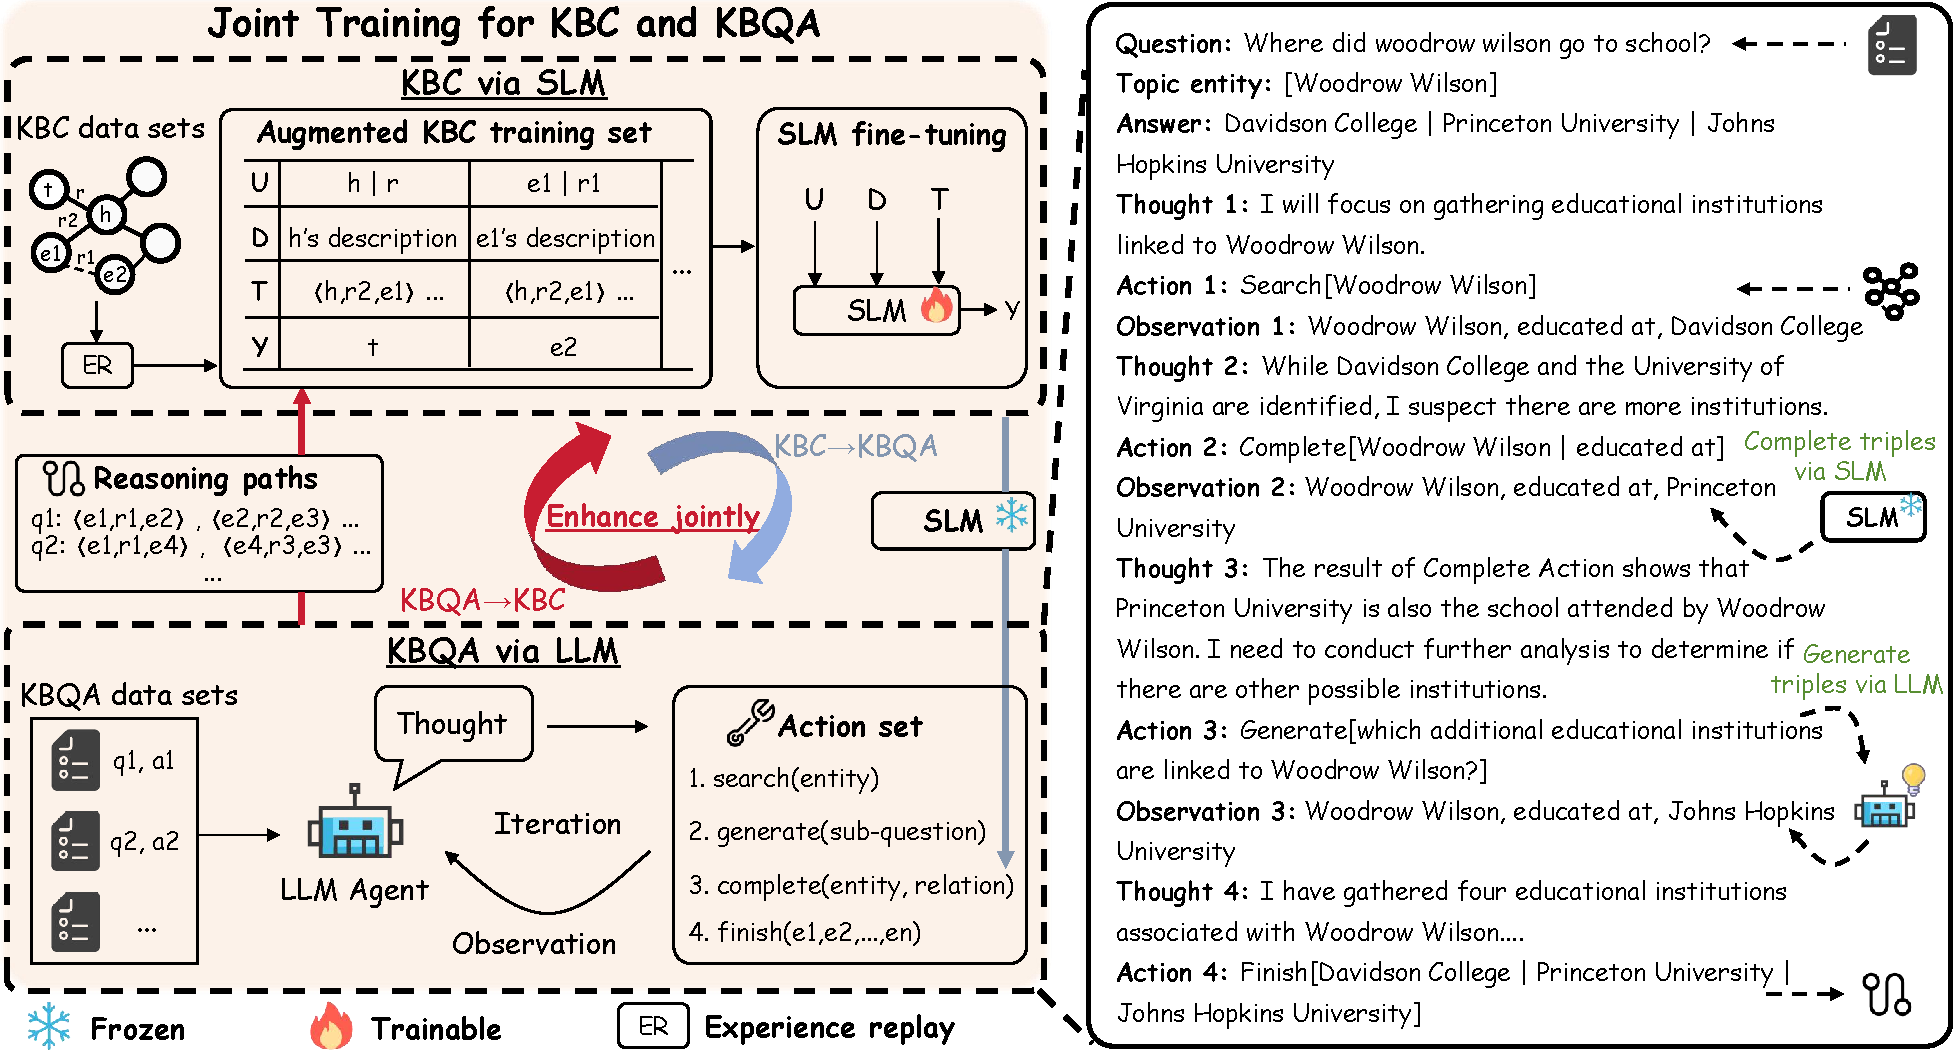
\includegraphics[width=0.56\textwidth]{image/img/Model_overview.pdf}}
%     \hspace{0.2em}
%     \subfigure[Inference]{
%         \label{model overview:subfig:twofunction}
%         \includegraphics[width=0.41\textwidth]{image/img/Inference.pdf}}
%     \caption{Model overview}\label{fig:init_mode}
%     \label{model overview}
% \vspace{-0.5em}
% \end{figure*}

